\documentclass[a4paper, 10pt]{ctexart} %中文支持
\usepackage{float}              %防止浮动元素浮动
\usepackage{rotating}           %旋转图片
\usepackage{amsfonts}           %对某一些字体之支持
\usepackage{mathrsfs}           %mathscr e.g.
\usepackage[]{amsmath}          %数学公式
\usepackage{amsthm}             %定义, 定理, 证明, 例子环境的支持
%使用方法:
%\newtheorem{environment name}{caption}
%比如 \newtheorem{example}{这是例子}
%效果 \begin{example} xxx \end{example} -> 这是例子 1 xxx
%proof就不需要了
\usepackage{graphicx}           %插入图片
\usepackage[left=1.25in,right=1.25in,top=1in,bottom=1in]{geometry}   %用来排版的
\usepackage[]{color}            %给部分文本上色的
\usepackage{algorithm}          %写伪代码的
%\usepackage{algorithmic}       %同上
\usepackage{algorithmicx}
\usepackage{algpseudocode}
\usepackage{minted}
\usepackage{amssymb}            %用来加入一些数学符号, 比如说 $\varnothing$
\usepackage{titlesec}
\usepackage{fontspec}           %不知道用来干嘛的
\usepackage{hyperref}           %生成可跳转的书签
% -------------------------------
\setmonofont{Ubuntu Mono}       %?
\usemintedstyle{custommanni}    %设置minted插入代码的风格
\titleformat*{\section}{\huge\bfseries}             %管理title的字体和大小
\titleformat*{\subsection}{\Large\bfseries}         %bfseries就是默认的字体.
\titleformat*{\subsubsection}{\large\bfseries}
% -------------------------------
\newtheorem{theorem}{Theorem}
\newtheorem{example}{Example}
\newtheorem{definition}{Definition}
\newtheorem{lemma}{Lemma}
\newtheorem{remark}{Remark}
\newtheorem{corollary}{Comment}
\newtheorem{proposition}{Proposition}
\pagestyle{plain}
\title{chapter 5: Greedy algorithm}
\author{You \and Me}
\date{date: Yesterday}
\begin{document}
\maketitle 
\tableofcontents
\section{what is greedy algorithm}
We say that divide and conquer divides a 
problem into some small 
but independent subproblem, while 
the dp divides the problem into some 
small subproblems that may overlap.
\begin{figure}
    \centering 
    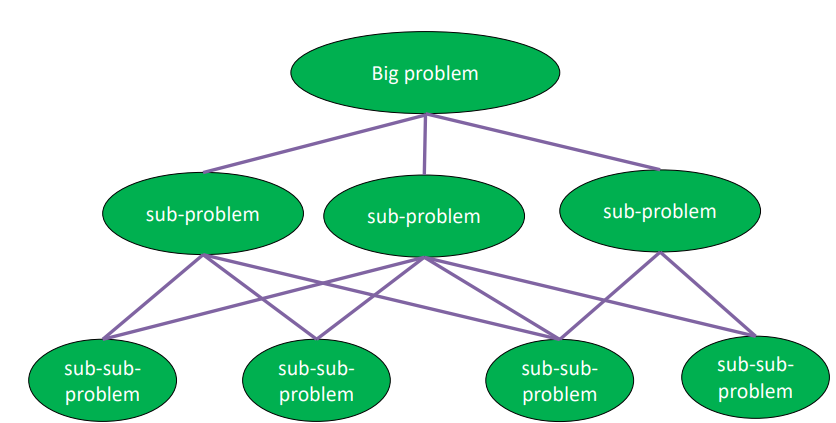
\includegraphics[scale = 0.5]{gd1.png}
    \caption{dp}
\end{figure}
figure 1 tells us about the structure of dp.

However, this greedy algorithm requires a 
high-demanding structure of the problem, which is called 
greedy 选择性, which can be described in figure 2.
\begin{figure}
    \centering
    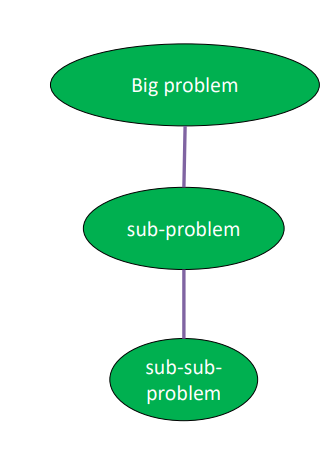
\includegraphics[scale = 0.5]{gd2.png}
    \caption{gd}
\end{figure}

The structure requires not only the optimal substrutrue but also 
requires the property that a big problem is based on one small 
problem. The algorithm is to 
decompose the solution to a complex problem into 
a sequence of operaitons of `locally optimal choice',
which extend the current local solution 
to a bigger one, till the solution can not 
be bigger.

Similar approuch can be applied to 
some other situation even 
if the resulted solution is not 
optimal.
\section{the basic principles of greedy}
The main idea of greedy algorithm can be described as follows
\begin{enumerate}
    \item The solution is a sequence of operations, while Divide and 
    conquer have some parrallel sequences of operations.
    \item Every operaitons makes a locally optimal choice.
    \item It requires proof of whether this approuch 
    leads to optimal solution.
\end{enumerate}
\begin{definition}
    The property that locally optimal choice leads 
    to globally optimal choice is called
    贪心选择性.
\end{definition}

\subsubsection{the comparison to dp}
\paragraph{dp} % (fold)
\label{par:dp}
Every choice is based on the solution to 
the subproblems. And it starts from button to top.
% paragraph dp (end)
\paragraph{greedy} % (fold)
\label{par:greedy}
Every choice is locally optimal, based on only the 
current situation. And it starts from top to bottom, with 
every choice decreasing the scale of the problems.
% paragraph greedy (end)
\section{任务安排问题}
\subsection{问题描述}
\begin{definition}
    $S$ 是 $n$ 个活动的集合, 这几个活动记为 $n$, i.e. $S = \{ 1,2,3,.. , n \}$. 
    每一个活动有开始时间和结束时间 记为 $\left[ s_i , f_i\right]$ \footnote{s for start, and f for fin}. 这几个活动不能有重叠,
    不能同时进行活动, 我们要求出最大相容活动集合 $A$, 即 $A$ 里面的活动不会发生矛盾
\end{definition}
\subsection{优化解的结构分析}
\begin{lemma}
    $S$ 的某个优化解包括活动 $1$
\end{lemma}
\begin{proof}
    设我们已知一个优化解 $A$, $k$ 是其第一个活动的下标, $j$ 是第二活动的下标

    $k=1$ 时候成立

    $k \ne 1$ 的时候, 有 $f_1 \le f_k \le s_j$, 其中 $f_k\le s_j$ 是因为相容.
    令 $B = A - \left\{ k\right\} \cup \left\{1\right\}$ 明显 $\left|  A \right|  =\left| B \right| $
\end{proof}
\begin{lemma}[优化子结构]
    设 $S = \left\{ 1, \cdots  ,n   \right\}$,
    并且包括活动 $1$ , 那么 $A ' = A - \{1\}$ 是 $S ' = \left\{ i \in S: s_i > f_1\right\}$ 的子问题的优化解
\end{lemma}
\begin{proof}
    使用反证法.

    如果说 $A'$ 不是 $S'$ 的优化解 (优化解在我这里 aka 最优解) , 设存在另一个 $A''$ 比 $A'$ 更优, 那么
    $A'' + \left\{1\right\}$ 比 $A$ 更优, 则矛盾. 

    一般优化子结构都是使用反证法.
\end{proof}
\begin{lemma}[符合贪心选择性]
    设 $S$ 是 $n$ 个活动, $l_i$ 是 $S_i = \left\{j \in S: s_j \ge f_{i-1}\right\}$ (特别的, $f_0 = 0$) 中具有最小结束时间的活动, 设 $A$ 是包含了活动 $1$ 的优化解, 那么 $A =\bigcup ^{k}_{i=1}\left\{ l_i\right\}$
\end{lemma}
\begin{proof}
    使用归纳法

    $\left| A \right| = 1 $ 时候, 结论成立

    $\left|  A \right|  < k$ 的时候, 假设成立; 那么 $\left| A \right|  =k $ 的时候, 考虑 $A' = A -{1}$, 由于引理2 和 假设: $A' = \bigcup _{i=2}^{k}\left\{ l_i\right\}$

    就有 $A = A'\cup \left\{1\right\} = \bigcup _{i=1}^{k} \left\{l_i    \right\}$
\end{proof}

算法正确性证明: 
\begin{itemize}
    \item 活动选择问题具有优化子结构
    \item 活动选择问题具有贪心选择性
    \item 算法按照贪心选择性计算优化解
\end{itemize}

\subsection{伪代码}
\begin{figure}[H]
    \centering
    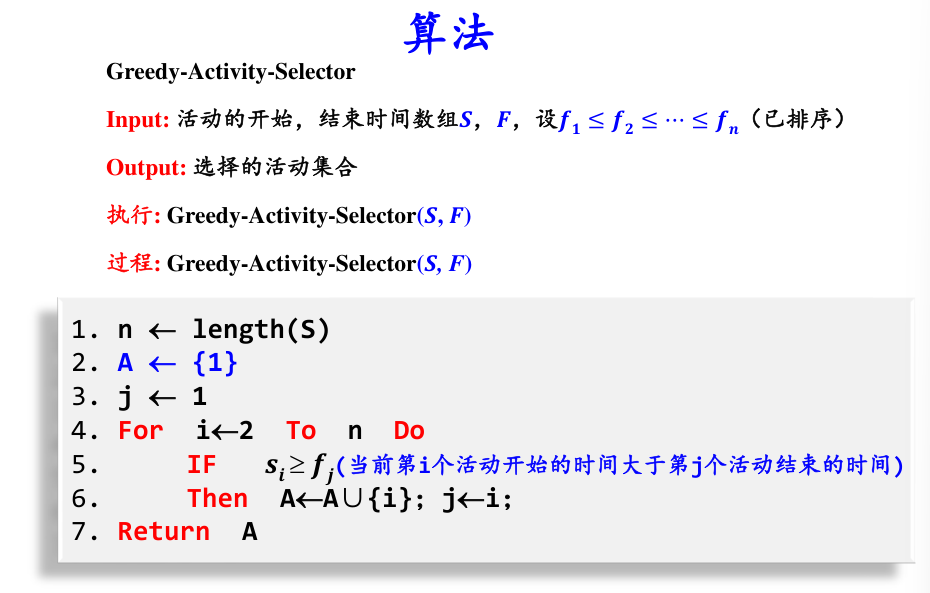
\includegraphics[scale =0.5]{6.png}
    \caption[]{活动优化伪代码}
\end{figure}
\begin{theorem}
    我们上面给出的算法能够产生最优解
\end{theorem}
\begin{proof}
    使用上面给出的三个引理就足以证明. 

    由于引理1, 我们选取活动 $1$, 这是合法的. 然后找出
    $S ' = {j: s _{j} \ge f_{1}}$ 的优化解. 是递归地来求解. 
\end{proof}
\subsection{复杂度分析}
不用怎么分析.
\[
T\left(n\right) =\Theta \left(n\right)
\]
上面只有一个循环. 

\section{哈夫曼编码问题}
\subsection{编码问题}
我们有很多种编码方法, 比如说什么ascii码什么的. 我们可以进行一个分类. 
\begin{enumerate}
    \item 二进制编码: 每一个编码使用一个二进制 sequence 来表示
    \item 固定长度编码: 每一个字符都是使用固定长度的 01 sequence 来表示.
    \item 可变长度编码: 经常出现的字符使用比较短的编码, 不经常出现的字符则相反. 这样传输效率会高一点.
    \item 前缀编码: 没有任何字符的编码是另一个字符编码的前缀. 不产生歧义, 理论上都得这样搞.
\end{enumerate}

在这里, 前缀编码是非常重要的, 哈夫曼编码就是其中一种. 我们说, 前缀编码可以表达为一棵树, 
其中一个 leaf 就是一个字符, 然后, 这个字符对应的一个 path 就是这个字符对应的编码. 
能够看出, 这个情况下, 没有任何字符的编码是另一个字符编码的前缀. 

我们可以简单证明一下, 如果说存在一个编码是另一个编码的前缀, 
那么这个编码对应的 path 是另一个 
path 的子集, 这说明那个节点并不是 leaf. 
毕竟是子集嘛. 那么产生矛盾.
\subsection{哈夫曼编码}
反正我们使用的是前缀编码, 每一个字母的编码不允许是另一个字母编码的前缀,
如果说有前缀, 不等长编码就没什么意义了. 哈夫曼编码就是这样的一个编码.

另一方面, 前缀编码实际上可以表示为二叉树, 每一个叶子节点就是一个编码, 
从根节点到叶子的路径对应着相应的编码.

我们计算代价:
$C$ 是字母, $\forall  c\in C $ , $p\left(c\right)$ 是 $c$ 出现的频率,
$d (c)$ 是其深度, 对应的是其编码的长度, 
代价的计算公式是 
\[
B\left(T\right) =\sum_{ c\in C}p(c) d(c)
\]

\subsection{问题描述}
\noindent 输入: 字母表 $C$, 以及对应的概率的表\\
输出: 具有最小 $B\left(T\right)$ 的前缀编码树, 即 $C$ 的哈夫曼编码树

\subsection{算法}
我们之前已经学过了, 但是还没有验证其正确性, 下面是一个使用了heap的算法, 非常简洁 (伪代码写得很难看, 所以还是用了点c, 不影响观看)
    \begin{minted}[mathescape, 
                   linenos, 
                   numbersep=5pt,
                   gobble=2,
                   frame=lines,
                   framesep=2mm]{c++}
    int main (){
        int n = |C|;
        init (Q, C); // initialize Q with C , Q is a heap
        for (int i = 1 ; i <= n-1 ; i++){
            z = AllocateNode (); // z 是一个节点. 
            left(z) = Extract-Min(Q); // 取出Q中最小的
            right(z)= Extract-Min(Q); // 同上
            x = left(z); // 将 z 的左边赋给 x
            y = right(z);
            p(z) = p(x) + p(y); // 给出 z 的概率. 
            insert (Q, z); // 将 z 插进 Q
        }
        return Q
    }
    \end{minted}
来看一下这个代码干了啥, 首先将字母表C塞进了heap Q 中, 关键字是其概率.
然后我们自底向上的求解, 拿出两个最小的, 合并一下, 塞回去. 循环 $n-1$ 次即可\footnote{这是因为每次合并是 $2 \to 1$, 所以说执行了 $n-1$ 次之后就只剩下一个节点了}. 实际上有点小问题, 因为到最后 Q 就只剩下一个点, return 的只是最终的代价. \footnote{我这里其实想错了, return的确实是完整的哈夫曼编码树.}
所以我们要将每次合并的操作进行一个记录.
\begin{figure}[H]
    \centering
    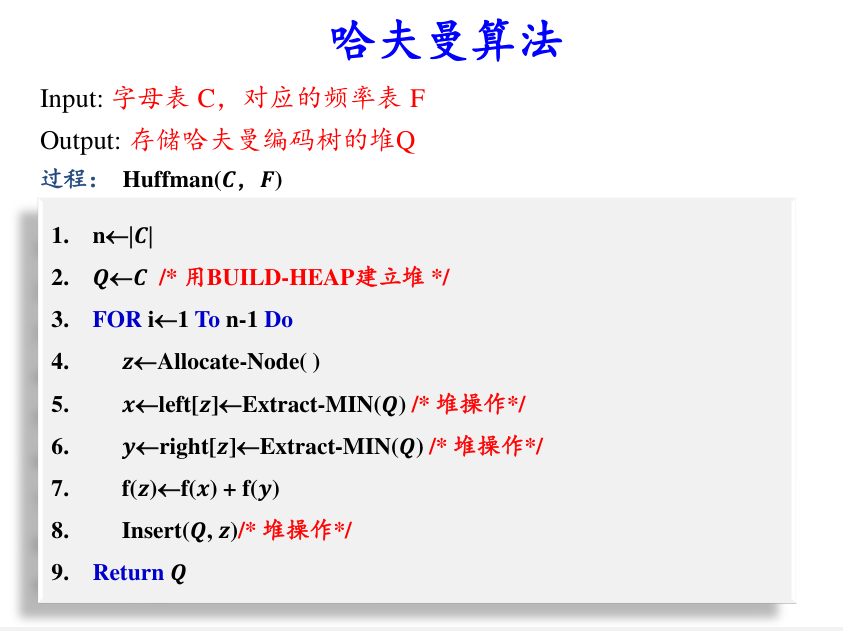
\includegraphics[scale = 0.5]{1.png}
    \caption[]{哈夫曼编码之伪代码}
\end{figure}

喂, 怎么记录啊, 你咋没说.
\subsection{算法复杂度分析}
\begin{figure}[H]
    \centering
    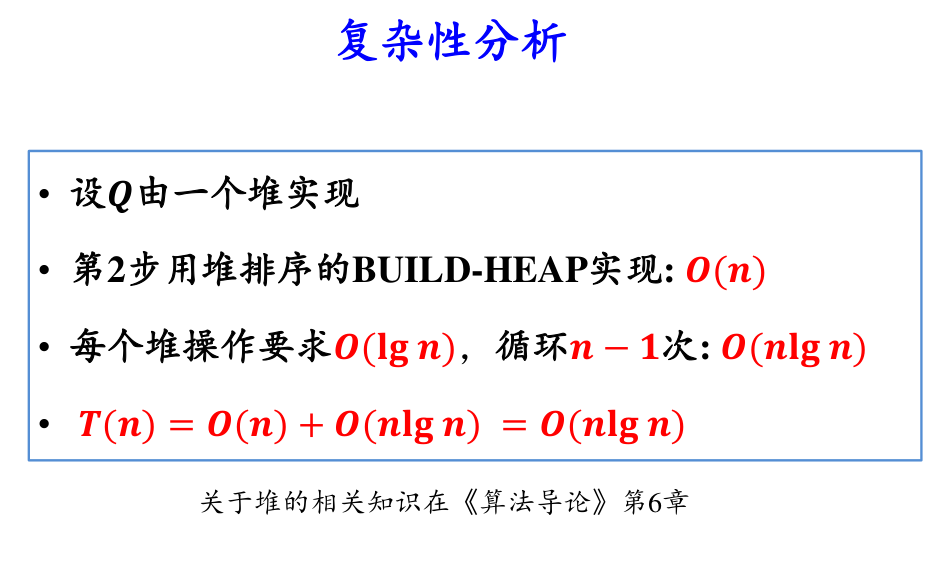
\includegraphics[scale= 0.5]{2.png}   
    \caption[]{哈夫曼编码 复杂性分析}
\end{figure}
\subsection{正确性证明}
\begin{lemma}[子结构]
    $C$ 的一个优化前缀树 $T$ 的子树 $T'$ 也是一个优化前缀树
\end{lemma}
\begin{proof}
    反证法, 这和前面的类似, 
    如果说 $T'$ 不是最优的, 就说明存在另一个 $T''$  代价更低, 
    于是就可以构造一个比 $T$ 更优的树
\end{proof}
\begin{lemma}[不知道叫什么]
    设 $T$ 是 $C$ 的一个优化前缀树, $x,  y$ 是两个相邻的叶子, $z$ 记作其父节点,
    将 $x,  y$ 视为一个点 $z$ , 并且 $p (z) = p(x)+ p\left(y\right)$
    
    则  $T'= T- \left\{ x, y \right\} $ 是 $C'$ 的优化前缀树. 其中 $C'=C - \left\{x, y\right\}+ \left\{z\right\}$ 
\end{lemma}
\begin{proof}
    明显有: $B\left(T\right)=  B\left(T'\right) + p\left(x \right)+ p \left(y\right)$
    
    考虑 $B\left(T\right) - B\left(T'\right)$ 来证明. 

    而后使用反证法, 如果说存在 $T''$ 是 $C'$ 的优化前缀树, 比 $T'$ 更优, 
    那么 $T'' + \left\{x, y\right\}$ 就\dots, 矛盾.
\end{proof}
\begin{lemma}[贪心选择性]
    设 $x , y $ 是 $C$ 中具有最小频率的两个字母, 则存在编码树使得 $x,y$ 编码具有相同长度, 并且仅最后一位不同, i.e. 是相邻的两个叶子
    \begin{figure}[H]
        \centering
        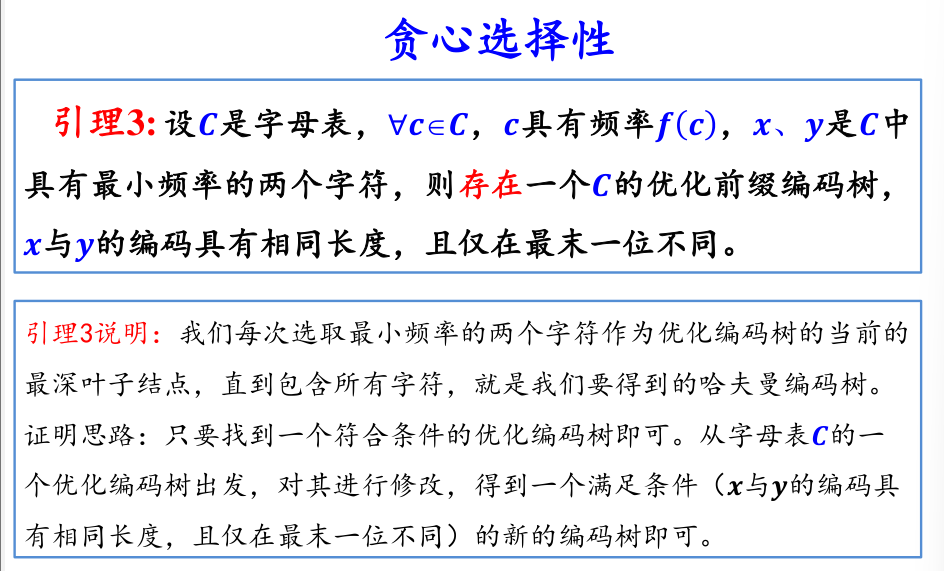
\includegraphics[scale = 0.5]{3.png}
        \caption[]{贪心选择性}
    \end{figure}
\end{lemma}
\begin{proof}
    对于一个编码树, 设其不满足 $x, y$ 相邻, 我们交换一下叶子节点, 构造出一个新的编码树, 并且是最优的即可.
    \begin{figure}[H]
        \centering
        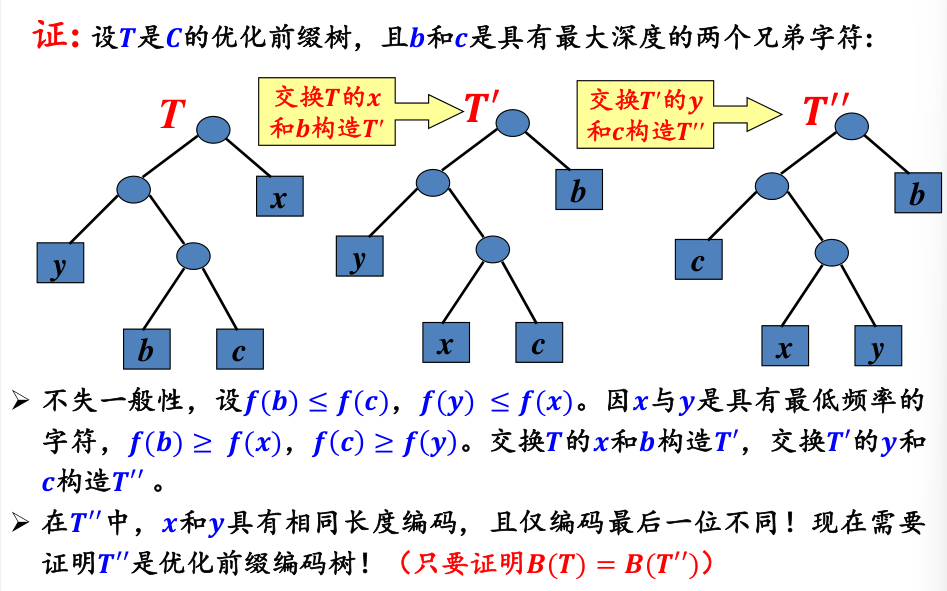
\includegraphics[scale = 0.5]{4.png}
        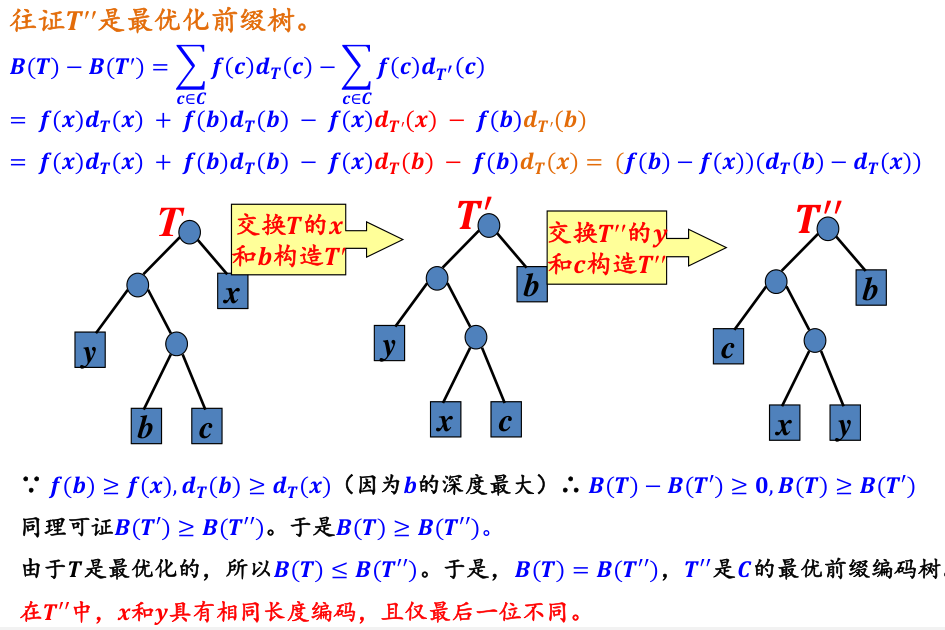
\includegraphics[scale = 0.5]{5.png}
        \caption{解}
    \end{figure}
    说实话, 这个非常明显, 不需要使用这么复杂的证明. 

    因为在底层的计数次数就越多, 既然 $p\left(x\right)$ 是最小的, 那么调换顺序之后, 
    权重变化值就是 
    \[
    \text{层数之差} \times \left( p(x) - p(a)\right) \le 0
    \]
    就是
    \[
    B \left(T''\right) \le B \left(T\right)
    \]
    然后既然 $B \left(T\right)$ 是最优的, 那么 $B \left(T''\right) = B\left(T\right)$, $T''$ 也是最优的.
\end{proof}

那么引理6为什么是证明了贪心选择性呢? 
这是因为它说明
\[
B \left(T\right)= B (T') + p (x) + p (y)
\]
并且这两个 $x, y$ 是能够知道的. 
\section{最小生成树}
问题引入, 比如说我们要修公路, 要使用在最短的公路将所有的站点链接起来. 
在互联网上也有应用.

\subsection{问题描述}
\begin{definition}[图的定义]
$G$ 是一个图, 其中 $V$ 是顶点集, $E$ 是边集, 一个边写为 $\left(u ,v\right), \quad u, v\in V$, 边可以有序, 也可以无序. 
\end{definition}
我们这里无序, 因为我们只涉及无向图 (目前).

\begin{definition}[生成树]
$G$ 的生成树记为 $T$, 为了某种意义上的严谨, 我们将 $T$ 写为 $\left(V_{t}, E_{t}\right)$, 符号用得并不是很熟练. 其中 $V_{t} = V$. 并且 $T$ 确实是一棵树. 
\end{definition}

正\footnote{这为什么要求是正的?}权重的无向简单图: 
我们可以为边赋上权值. 总之我们这里只涉及正权值的图. 

简单图: 如果说两个顶点之间的边小于等于 $1$ 条, 则称这个图是简单图 (应该把, 定义有点忘了)

我们现在问题就是:

$\mathbf{Input}$ : 给定一个图 $G = \left(V ,E\right)$

$\mathbf {Output}$ : 给出这个图的最小生成树, i.e. 权重和最小的生成树.
\subsection{graph cut}
\begin{definition}[graph cut]
    $S \subset V$, 那么 $\left\{ S , V- S\right\}$ 是 $V$ 的一个划分. 这就是一个图割
\end{definition}
\begin{definition}[三个概念]
    $(u,v)$ 是一个横跨边, 如果 $u \in S,v \in V-S$ 

    $A$ 是 边集 的子集, $A \subset E$, $S$ 尊重 $A$, 如果 $\forall  e \in A \implies e$ 不是横跨边. 

    $e$ 是轻量型边, 如果 $e$ 是横跨边中权值最小的那个.
\end{definition}

\begin{lemma}
    $E' \subset E$, 如果存在一个 cut 尊重 $E'$ , 如果
    \begin{itemize}\setlength\itemsep{-0.2em}
        \item[1.] 存在包含了 $E'$ 的最小生成树. 
        \item[2.] $\left(u ,v\right)$ 是轻量型边. 
    \end{itemize}
    则有: 存在包含了 $E' \cup \left\{ \left( u,v\right)\right\}$ 的最小生成树. 
\end{lemma}
\begin{proof}
    设已知有一个树 $T'$ 包含了这个 $E'$ . 我们断言, $T'$ 中仅包含了一个横跨边. 
这是因为, 如果说不包含横跨边, 那么边的数量为 $\left| V \right|  - 2$ 不可能是树. 又如果说, 有两个横跨边, 
则边的数量为 $\left| V \right|  $ 一定存在圈, 则不是树.

我们能够构造一个最小生成树, 只需要, 将这个横跨边删去, 再加上轻量型边. 

明显有: $B \left(T''\right) \le B \left(T'\right)$ 因为是轻量型边嘛, 但同时 $T'$ 是最小生成树.
所以说 $T''$ 也是最小生成树.
\end{proof}
\subsection{Prim 算法}
\subsubsection{图解过程}
鸽了
\subsubsection{伪代码}
初始化相当于加入了初始节点 $r$, 然后继续加边. 

这边第1-3都是一个初始化. 
key 向量储存的是某节点 $v$ 的轻量型边的权重. (如果 $v$ 已经在树里面了该怎么办?)

$\pi  $ 储存 $v$ 的父节点, 我们就是根据这个构造解. 

第5行没看懂.

6-7行也没看懂, 这是在干什么? 为什么这个循环能够找出轻量型边的端点? 

我这个key是用来干什么的? 是用在 \verb|Extract-Min| 这个函数上吗?

\begin{figure}[H]
    \centering
    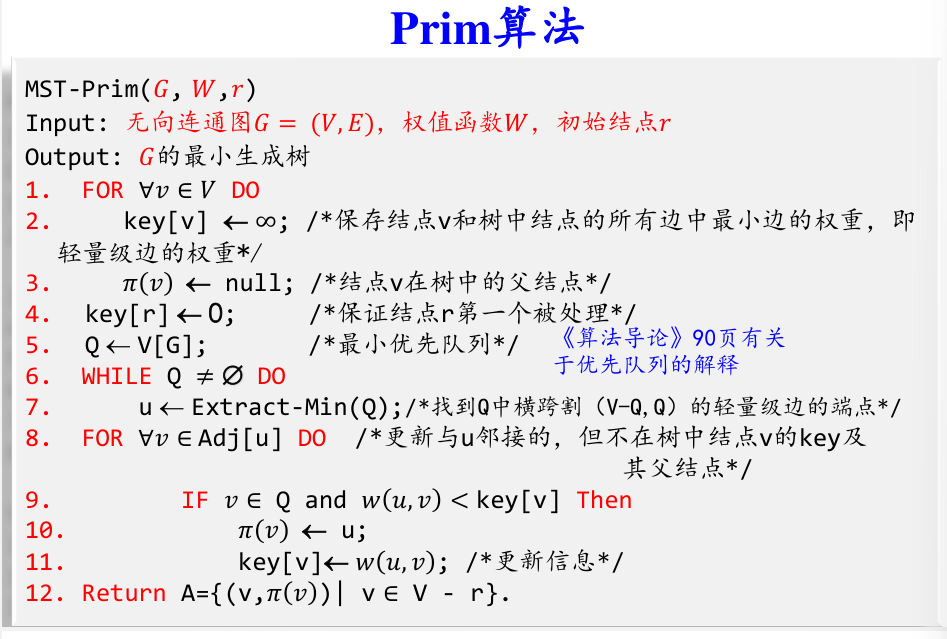
\includegraphics[scale = 0.5]{7.png}
    \caption[]{Prim 算法}
\end{figure}

这算法是真几把牛逼. 看不懂
\subsubsection{正确性证明}
使用归纳法. 
\begin{enumerate}
    \item 
基本情况: 增加 $0$ 条边的时候, 边集为空, 确实是最小生成树的一部分.
\item
归纳步骤: 
对于 $S$ 已经是最小生成树的一部分, 
那么我们加一条边 (轻量型边) 也是最小生成树的一部分. 
\item
结论: 每次得到的边集都是最小生成树的一部分, 当所有的点都加进去了, 得到的是最小生成树.
\end{enumerate}


\subsection{Kruskal 算法}
加入轻量型边. 也称为 ``加边法'' (佛了, 难道prim就不加边了吗). 
我们先是将单独一个顶点作为一棵树, 形成一个森林. 

划分是森林中的每棵树, 依然是找出轻量型边, 然后合并两颗树. 然后继续加边.

但在实现过程中, 会有更新某某数组的情况出现. 
\subsubsection{伪代码}
废话不多说, 直接来看伪代码

注: $S \subset E$, \verb|union| 是将 $u,v$ 所在的树连在一起, 合并为一棵树.

\begin{figure}[H]
    \centering
    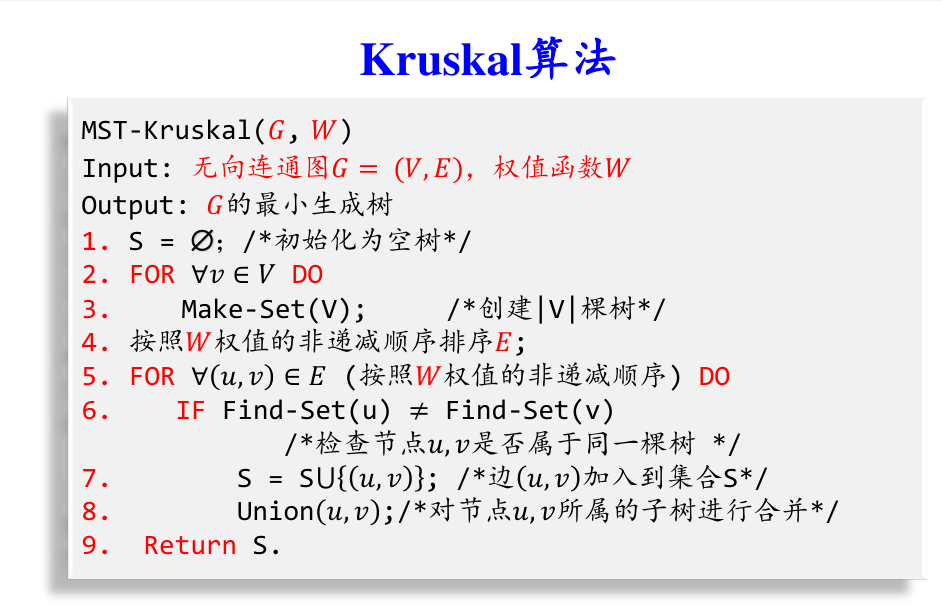
\includegraphics[scale = 0.5]{8.png}
    \caption{Kruskal 算法之伪代码}
\end{figure}

这里我们能够看到为什么说 \verb|Kruskal| 是加边法了. 输出都是边, 不需要特殊的存储信息的过程.
\subsubsection{复杂度分析}

\begin{itemize}
    \item 令 $\left| V \right|  =n , \left| E \right|  =m$
    \item 4 需要时间 $O \left( m \log m\right)$
    \item 2-3 需要执行 $O \left(n\right)$ 个 \verb|Make-set| 操作. 
    \item 5-8 需要 $O \left(m\right)$ 个 \verb|Find-Set| 和 \verb|Union| 操作. 需要时间 $O \left( \left(n+m\right) \alpha (n)\right)$ \footnote{为什么??}
    \item $m \ge n-1$, $\alpha \left(n\right) = \log  n = \log m$ \footnote{这又是什么?}
    \item 总的时间复杂度就是 $O\left(m \log  m  \right)$
\end{itemize}
\begin{figure}
    \centering
    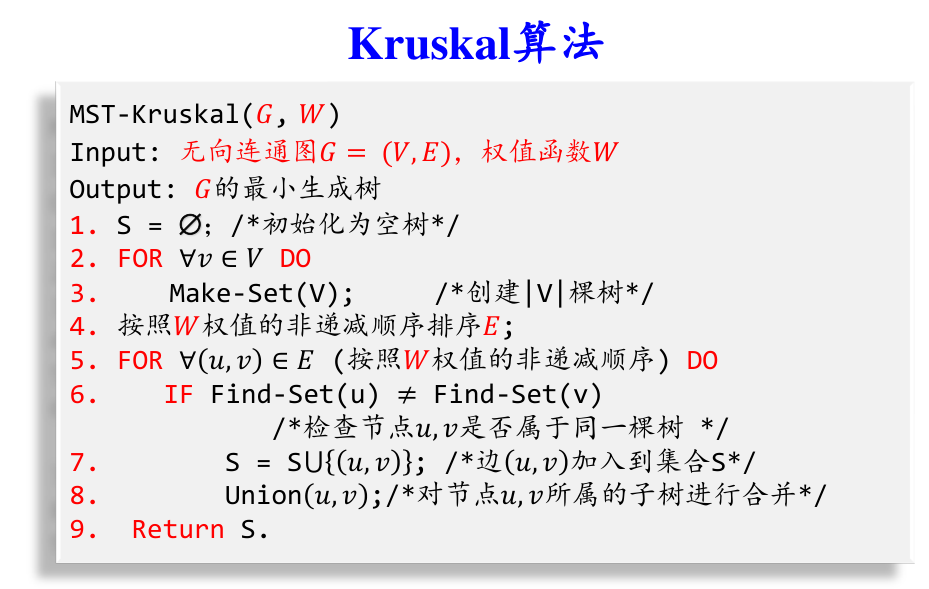
\includegraphics[scale = 0.5]{9.png}
    \caption{Kruskal算法之伪代码}
\end{figure}
\end{document}